\subsection{Data and Labelling}
\label{data}
\subsubsection{KITTI Dataset}
The KITTI 2D/3D object detection challenge is dedicated to autonomous driving and releases a dataset containing 7481 images for each one of 4 cameras and their associated labels and calibrations \cite{Geiger2012CVPR}. The dataset covers scenarios of city, residential, road, campus, and person. We only use the images taken by the left colour camera. The example image is shown in Figure \ref{figure:kitti_image}. The associated labels are show in Table \ref{kitti_lable}. The calibration is given as transformation matrix.

\begin{figure}[h]		
	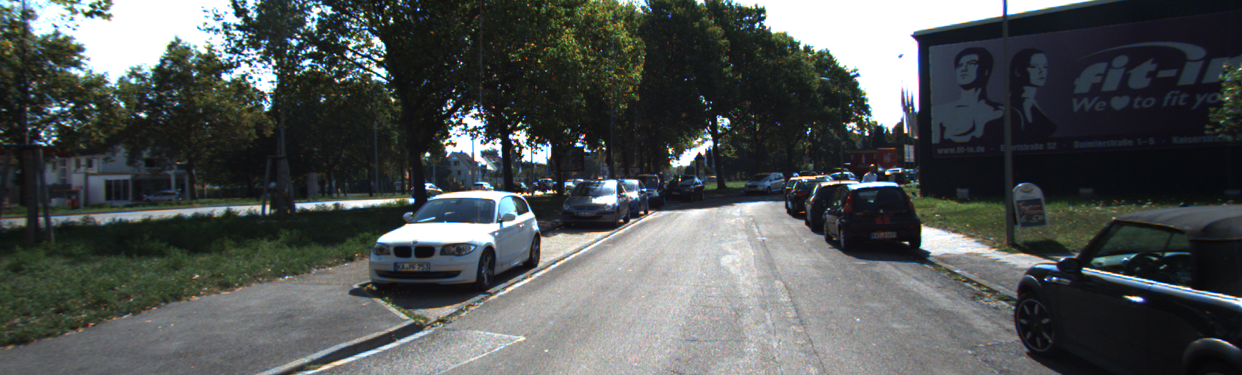
\includegraphics[width=1\textwidth]{000010.png}
	\caption{Example image from KITTI dataset captured by the left colour camera}
	\centering
	\label{figure:kitti_image}
\end{figure}

\begin{table}[h]
	\centering
	\caption{Label specification of KITTI dataset}
	\label{kitti_lable}
	\resizebox{\textwidth}{!}{%
		\begin{tabular}{|c|c|l|}
			\hline
			\#Values & Name        & Description                                                                                                                                                             \\ \hline
			1        & type        & \begin{tabular}[c]{@{}l@{}}Type of object: \\ 'Car', 'Van', 'Truck', 'Cyclist', 'Tram', 'Pedestrian', \\ 'Person\_sitting',  'Misc' or 'DontCare'\end{tabular}          \\ \hline
			1        & truncated   & \begin{tabular}[c]{@{}l@{}}Float from 0 (non-truncated) to 1,\\ indicating the extent of the object out of the image\end{tabular}                                       \\ \hline
			1        & occluded    & \begin{tabular}[c]{@{}l@{}}Integer indicating occlusion state: \\ 0 = fully visible, 1 = partly occluded, \\ 2 = largely occluded, 3 = unknown\end{tabular}             \\ \hline
			1        & alpha       & Observation angle of object, ranging {[}-pi..pi{]}                                                                                                                      \\ \hline
			4        & bbox        & \begin{tabular}[c]{@{}l@{}}2D bounding box of object in the image (0-based index): \\ contains left, top, right, bottom pixel coordinates ($x_1$, $y_1$, $x_2$, $y_2$)\end{tabular} \\ \hline
			3        & dimensions  & 3D object dimensions: height, width, length (in meters)                                                                                                                 \\ \hline
			3        & location    & 3D object location x,y,z in camera coordinates (in meters)                                                                                                              \\ \hline
			1        & rotation\_y & Rotation ry around Y-axis in camera coordinates {[}-pi..pi{]}                                                                                                           \\ \hline
		\end{tabular}%
	}
\end{table}

\subsubsection{3D Vehicle Dataset}
This dataset is intended to encode the diversity of vehicles by means of type, dimension, and chassis shape. It is created based on a selected subset of synthetic 3D CAD models\cite{NIPS2012_4562}. We only include the well-aligned and  symmetrical models, and also take the dimension and type into consideration. We classify all the models into six categories: Mini, Hatchback, Sedan, SUV, Wagon, and Van. And for each category,  subcategories are marked out according to their dimensions and shapes in order to make a refined selection.  The statistic of dimensions is well distributed and each existing car can be classified into one category exclusively.

\begin{figure}[h]		
	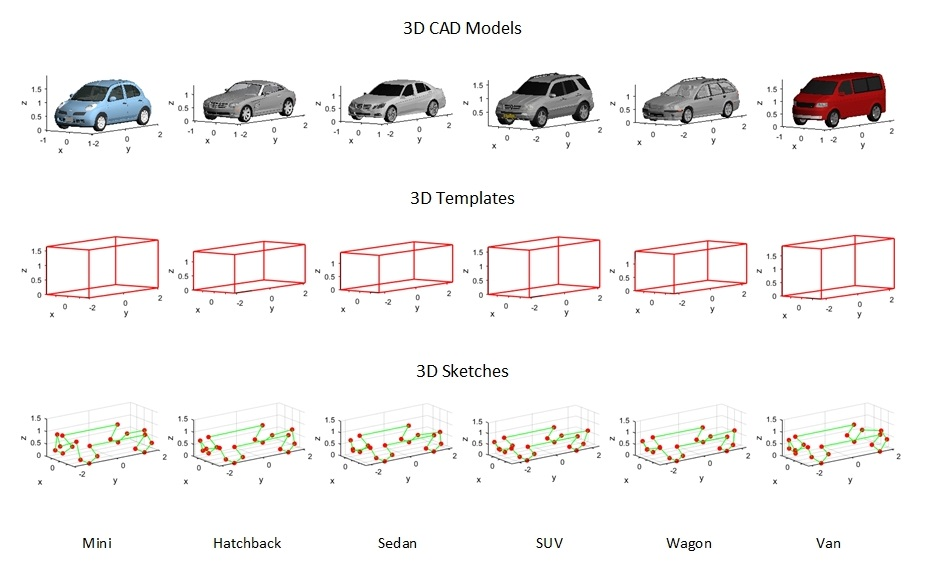
\includegraphics[width=1\textwidth]{vehicle_dataset.jpg}
	\caption{Six vehicle categories of the 3D vehicle dataset. Each vehicle model is associated to a 3D CAD model, a 3D template, and a 3D sketch.}
	\centering
	\label{figure:vehicle_dataset}
\end{figure}

Our final dataset consists of 54 valid vehicle models. Each vehicle model has a 3D CAD model, a 3D template, and a 3D sketch correspondingly, as shown in Figure \ref{figure:vehicle_dataset}. All these three representation are aligned in canonical view and share an identical object coordinate system. The CAD models are created based on real vehicles and have all the geometry information with them. The 3D templates represent the vehicles' dimensions. The 3D template associated to the 3D model $k$ is denoted as $t_k = (h_k, w_k, l_k)$ where $h_k, w_k$ and $l_k$ represent the height, width, and length of the model respectively. 

The  3D sketches indicate the chassis shapes. Each 3D sketch consists of 20 characteristic points around the chassis with each point denoting one part of the vehicle. So the $k^{th}$ sketch is denoted as $S_k^{3d}  = (p_1, p_2, ... p_{20})$, where $~p_i = (x_i, y_i, z_i)$. The reason why we choose the points around chassis as feature points is that their geometric relationship is more stable than points in other places. Because the chassis part is more about functionality than appearance attraction compared to other parts of the vehicle,  \eg the upper part. In this way, the sketches can be more universal so that they can represent a wider range of vehicles, which reduces the number of models required and further increases the computational efficiency. 

In order to create the 3D sketches, we implement a labelling tool, shown in Figure \ref{figure:label_cad}. It is capable to label the 3D coordinates for all the characteristic points associated to each vehicle.[\tbd  should it be elaborated in detail]

\begin{figure}[h]		
	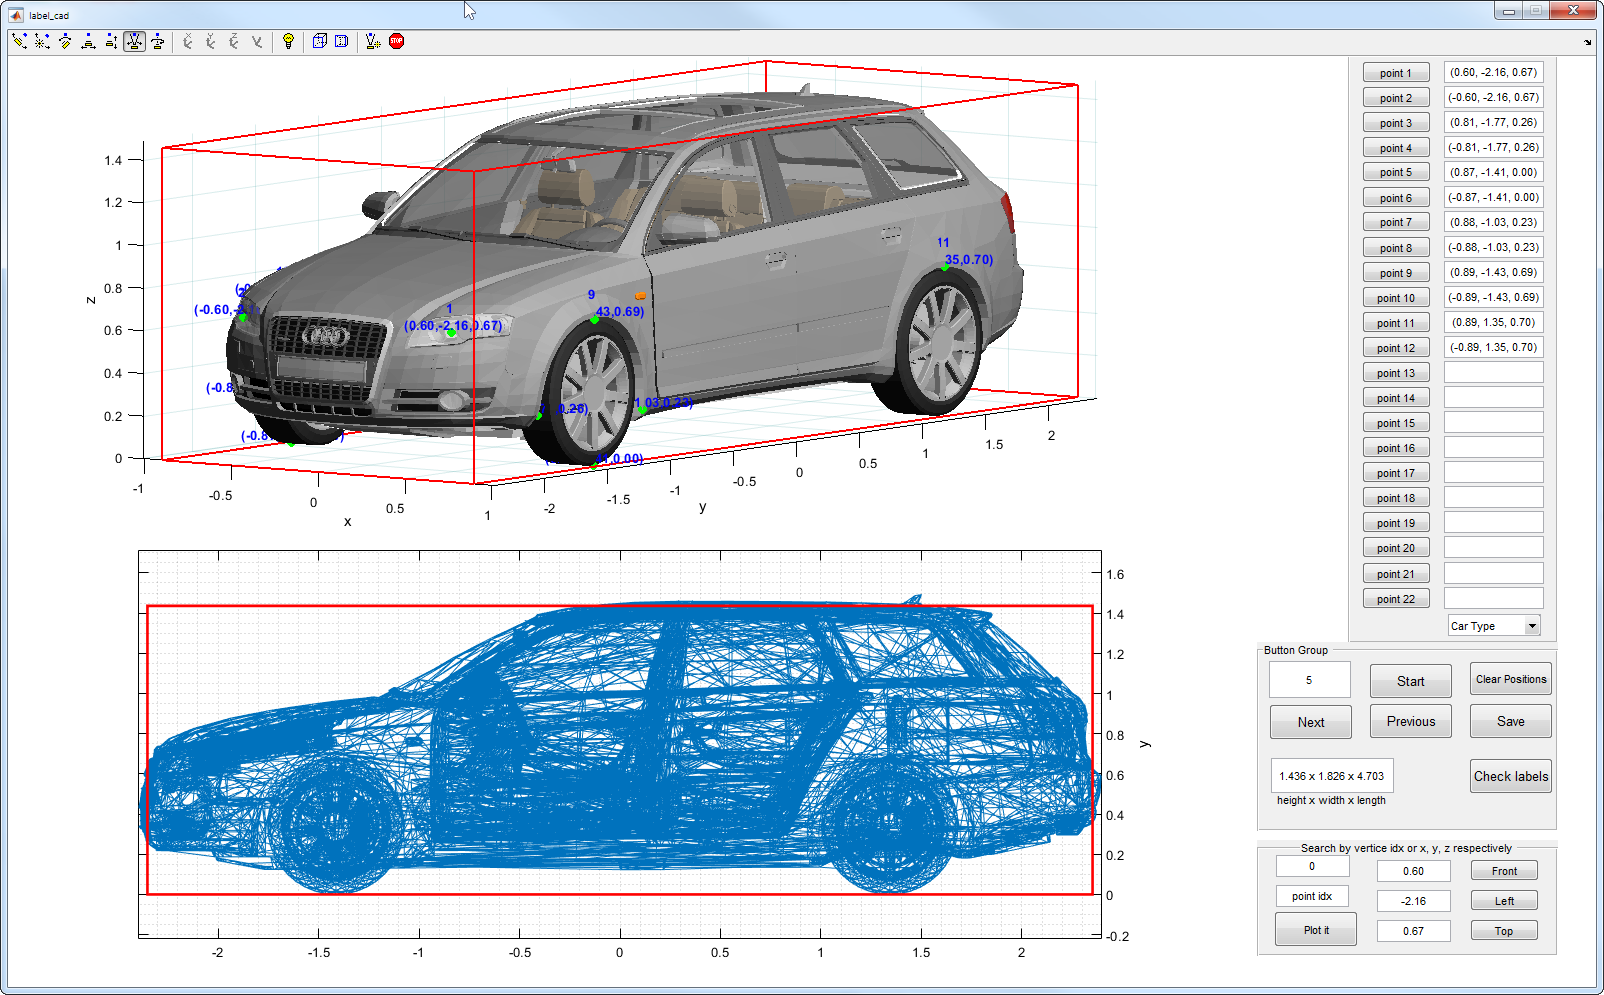
\includegraphics[width=1\textwidth]{label_cad.png}
	\caption{Labelling tool for 3D sketches}
	\centering
	\label{figure:label_cad}
\end{figure}

\subsubsection{Labelling for KITTI Dataset}

Our approach requires three extra kinds of labels to training the CVT Network, \ie 2D coordinates and visibility property of characteristic points and template proximity, as shown in Table \ref{new_label}.  Labelling is never a trivial task. Due to the demanding workload of manual labelling and the cases where it is almost impossible to label the small vehicles in image manually, we propose an automatic label generation method. It is able to make use of the 3D vehicle dataset and the KITTI dataset to generate these three additional kinds of ground truth.

\begin{table}[h]
	\centering
	\caption{Specification of three additional labels}
	\label{new_label}
	\resizebox{\textwidth}{!}{%
		\begin{tabular}{|c|c|l|}
			\hline
			\#Values & Name        & Description                                                                                                                                                             \\ \hline
			2x20        & 2D coordinate  & $(x, y)$, location of 20 characteristic points in image coordinates                                                                                                                \\ \hline
			1x20        & visibility    & \begin{tabular}[c]{@{}l@{}}Integer indicating visibility property of each point: \\ 0 = visible, 1 = occluded, \\ 2 = self-occluded, 3 = truncated\end{tabular}    \\ \hline
			3x54        & template proximity & \begin{tabular}[c]{@{}l@{}} A vector $\mathit{T_{i}}$ represents the dimension ratios \\ between each model and the vehicle  \end{tabular}   \\ \hline
		\end{tabular}%
	}
\end{table}


\paragraph{2D Coordinates}

2D coordinates of key points of each vehicle in image coordinates is generated by projecting the 3D sketch of this vehicle to the image. The vehicle's 3D sketch is selected via template-matching, \ie the best-matching sketch is the one whose associated template is closest to the vehicle's dimensions. The 3D-2D projection is performed based on the given intrinsic and extrinsic parameters, as shown in Figure \ref{3D_2D_projection}. The intrinsic parameters are given as calibration by KITTI and the extrinsic parameters are given as 3D object dimensions and rotation ry in KITTI labels. KITTI makes a simplified assumption here that the vehicle only rotates around the yaw axis but not roll or pitch axis. One example of the labelled 2D coordinates is shown in Figure \ref{visibilie_eg}.

\begin{figure}[h]		
	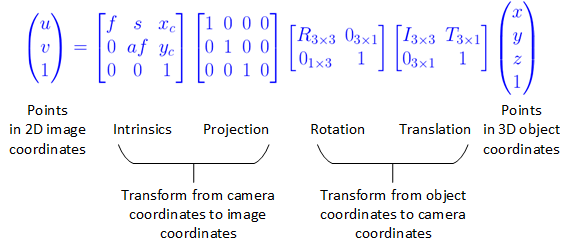
\includegraphics[width=1\textwidth]{projection_matrix.png}
	\caption{3D-2D projection}
	\centering
	\label{3D_2D_projection}
\end{figure}

\begin{figure}[h]		
	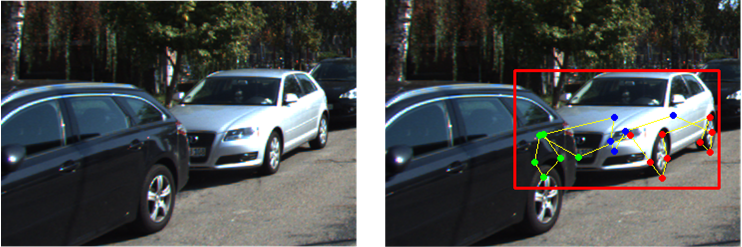
\includegraphics[width=1\textwidth]{visibilie_eg.png}
	\caption{Example of 2D coordinates and visibility of one vehicle. The left image is one patch of KITTI image. The left image is the one after labelling. The points indicate the 2D coordinates and the color indicates the types of visibility: red for visible, green for occluded, and blue for self-occluded.}
	\centering
	\label{visibilie_eg}
\end{figure}



\paragraph{Visibility}

As an example of the labelled visibility shows in Figure \ref{visibilie_eg}, the visibility property of characteristic points is classified into four scenarios: 

\begin{enumerate}[\hspace{0.4cm} i.]
	\itemsep-0.5em 
	\item Visible if the point can be seen directly;
	\item Occluded if the point is occluded by other objects;
	\item Self-occluded if the point is blocked out by the vehicle itself;
	\item Truncated if the point exceeds the boundaries of the image. 
\end{enumerate}

\begin{figure}[h]		
	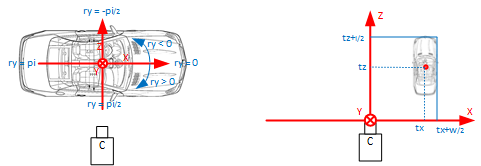
\includegraphics[width=1\textwidth]{visibility_imp.png}
	\caption{Visibility labelling mechanism. The left image shows the rotation ry in the camera coordinate system, which helps distinguish visible or self-occluded case. The left image shows the location of the vehicle in the camera coordinate system, which helps defined the occluded situation.}
	\centering
	\label{visibility_imp}
\end{figure}

The visibility of each point is determined by its position, \ie the 2D coordinate in image.  Being visible or self-occluded is distinguished by means of rotation ry of each vehicle. As the right plan sketch in Figure \ref{visibility_imp} shows, the rotation ry can indicate unambiguously which faces of the vehicle are facing to or away from the camera. If the points are on the observable faces, they  are labelled as visible,  otherwise they are classified as self-occluded. Occluded case happens when the 2D coordinate of the point falls into the 2D bounding box of a former object. The object is defined as former when it locates in the region enclosed by the axes and two solid blue line in the left schematic plot of Figure \ref{visibility_imp} if the vehicle is on the first quartile.  And when the vehicle is on the second quartile, it's just a mirrored case. Truncated is defined that its 2D coordinate exceeds the boundaries of the image. The size of KITTI images are determined which makes it easy to implement. The truncated property has the highest priority, the occluded underlies , the self-occluded or the visible is considered at last.


\paragraph{Template Proximity}
\label{template}

Template proximity of one vehicle is encoded as a vector $\mathit{T_{i}}$ which is defined as $\mathit{T}_i = \{r_k\}_{k \in \{1,.., K\}}$, where $\mathit{K}$ denotes the number of 3D vehicle models and  $r_k~=~(r_h,r_w,r_l)$ corresponds to three scaling ratios between the dimensions (\ie height, width, and length) of each model and the vehicle's respectively. The vector $\mathit{T_{i}}$ represents the similarity between each model and the vehicle. The most similar model is the one whose $r_k$ is closest to $(1, 1, 1)$.

\subsubsection{Notations}
In sum, based on the KITTI image and 3D vehicle models, each vehicle can be defined by seven critical attributes:
\[  \{D, B^{2d}, ~B^{3d}, ~C^{2d}, ~C^{3d}, ~V, ~T\}  \]
$D = (h, w, l)$ represents the dimensions of the vehicle. $B^{2d} = (c_u, c_v, w, h)$ defines the 2D bounding box in image with $(c_u, c_v)$ denoting its center,  $w$ for its width and $h$ for its height. $B^{3d} = (o, \theta, d)$ where $o = (c_x, c_y, c_z)$ is the center, $\theta$ is the rotation ry around the yaw axis, and $d = (w, h, l)$ is its dimensions. $C^{2d}  = \{(u_i, v_i)\}_{i \in \{1, ...,20\}}$ represents the 2D part coordinates in image plane, while $C^{3d}  = \{(x_i, y_i, z_i)\}_{i \in \{1, ...,20\}}$ denotes the 3D part coordinates in world coordinate system. $V = \{v_i\}_{i \in \{1, ...,20\}}$ is the visibility for all the characteristic points in the vehicle.  $T = \{{(r_{h},r_{w},r_{l})}_k\}_{k \in \{1, ...,54\}}$ is the template proximity vector.
